% Created 2023-02-11 Sat 22:26
\documentclass[9pt, b5paper]{article}
\usepackage{xeCJK}
\usepackage[T1]{fontenc}
\usepackage{bera}
\usepackage[scaled]{beraserif}
\usepackage[scaled]{berasans}
\usepackage[scaled]{beramono}
\usepackage[cache=false]{minted}
\usepackage{xltxtra}
\usepackage{graphicx}
\usepackage{xcolor}
\usepackage{multirow}
\usepackage{multicol}
\usepackage{float}
\usepackage{textcomp}
\usepackage{algorithm}
\usepackage{algorithmic}
\usepackage{latexsym}
\usepackage{natbib}
\usepackage{geometry}
\geometry{left=1.2cm,right=1.2cm,top=1.5cm,bottom=1.2cm}
\usepackage[xetex,colorlinks=true,CJKbookmarks=true,linkcolor=blue,urlcolor=blue,menucolor=blue]{hyperref}
\newminted{common-lisp}{fontsize=\footnotesize} 
\author{deepwaterooo}
\date{\today}
\title{Emacs Configuration}
\hypersetup{
  pdfkeywords={},
  pdfsubject={},
  pdfcreator={Emacs 28.1 (Org mode 8.2.7c)}}
\begin{document}

\maketitle
\tableofcontents


\section{TODOs: tracing bugs of emacs 28.1}
\label{sec-1}
\section{Updates}
\label{sec-2}
\subsection{configuration for pdf-tools packages}
\label{sec-2-1}
\begin{itemize}
\item pdf viewer noter <==> Skim bi-directional linking configuration on the way, most emacs work is done. Need to learn how to use them though.
\end{itemize}

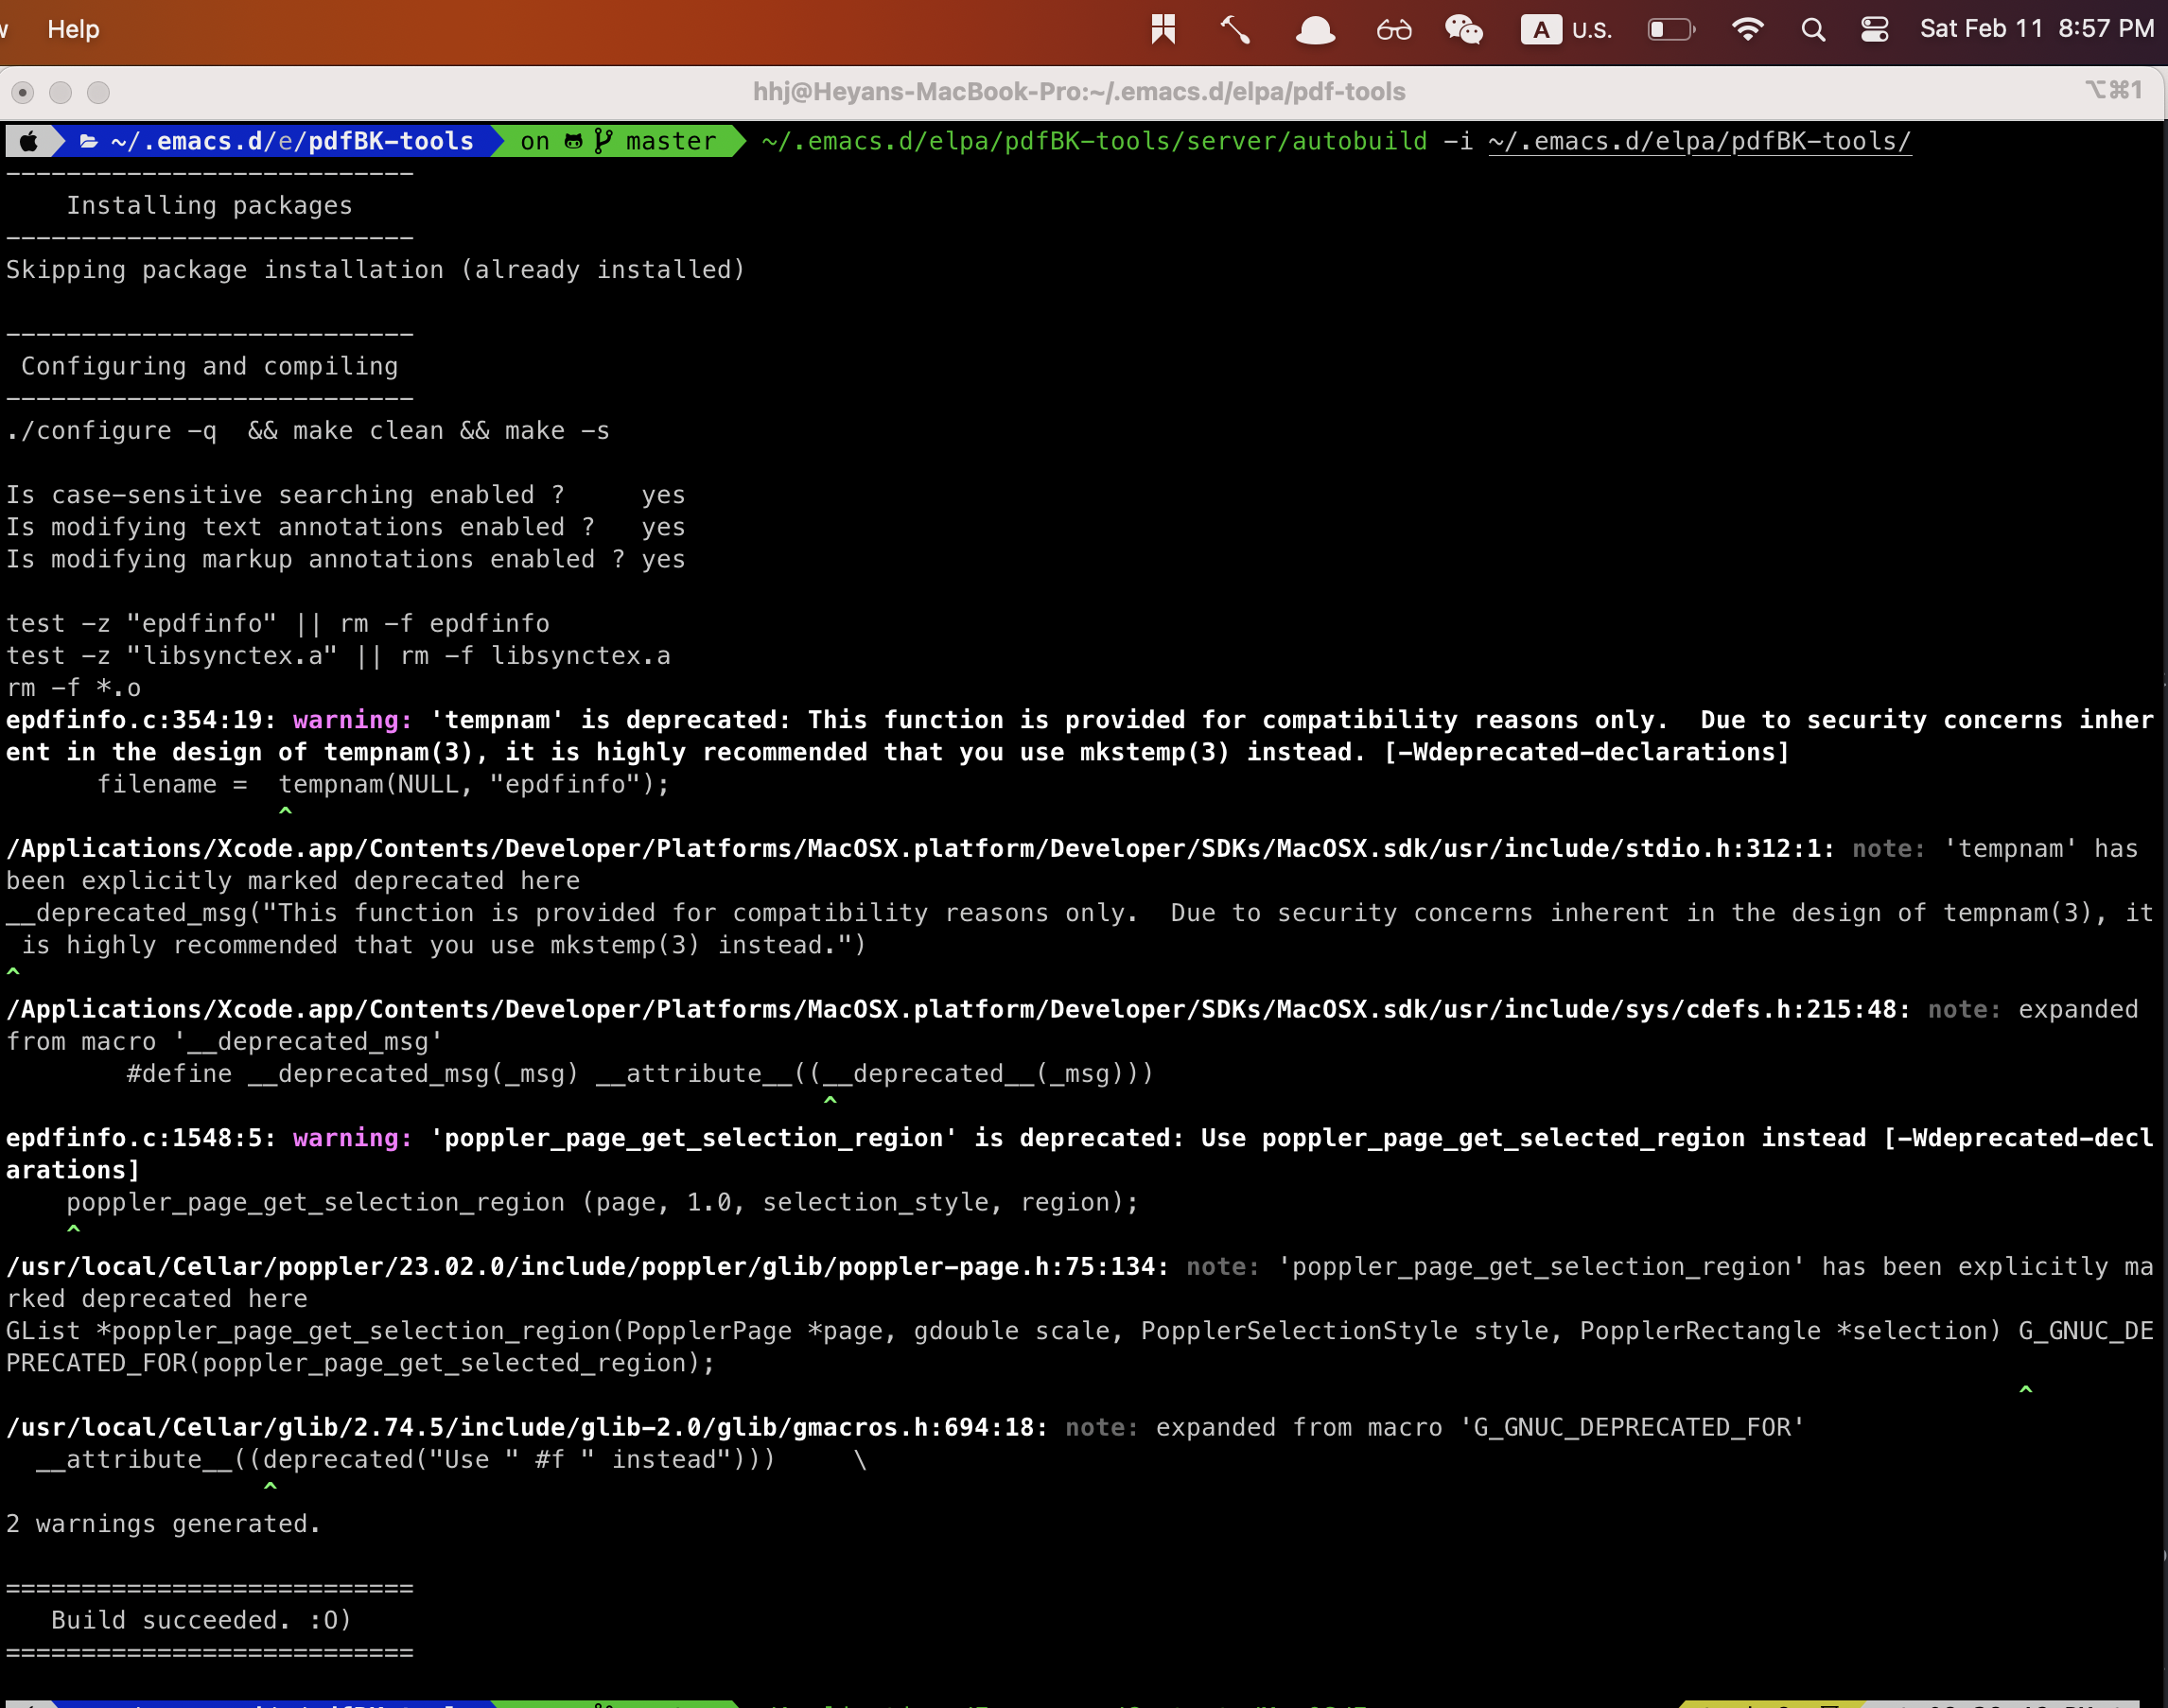
\includegraphics[width=.9\linewidth]{./pic/Snipaste_2023-02-11_20-57-40.png}
\begin{itemize}
\item It has to be configured for M1. But I am still not getting any .tar file yet. 

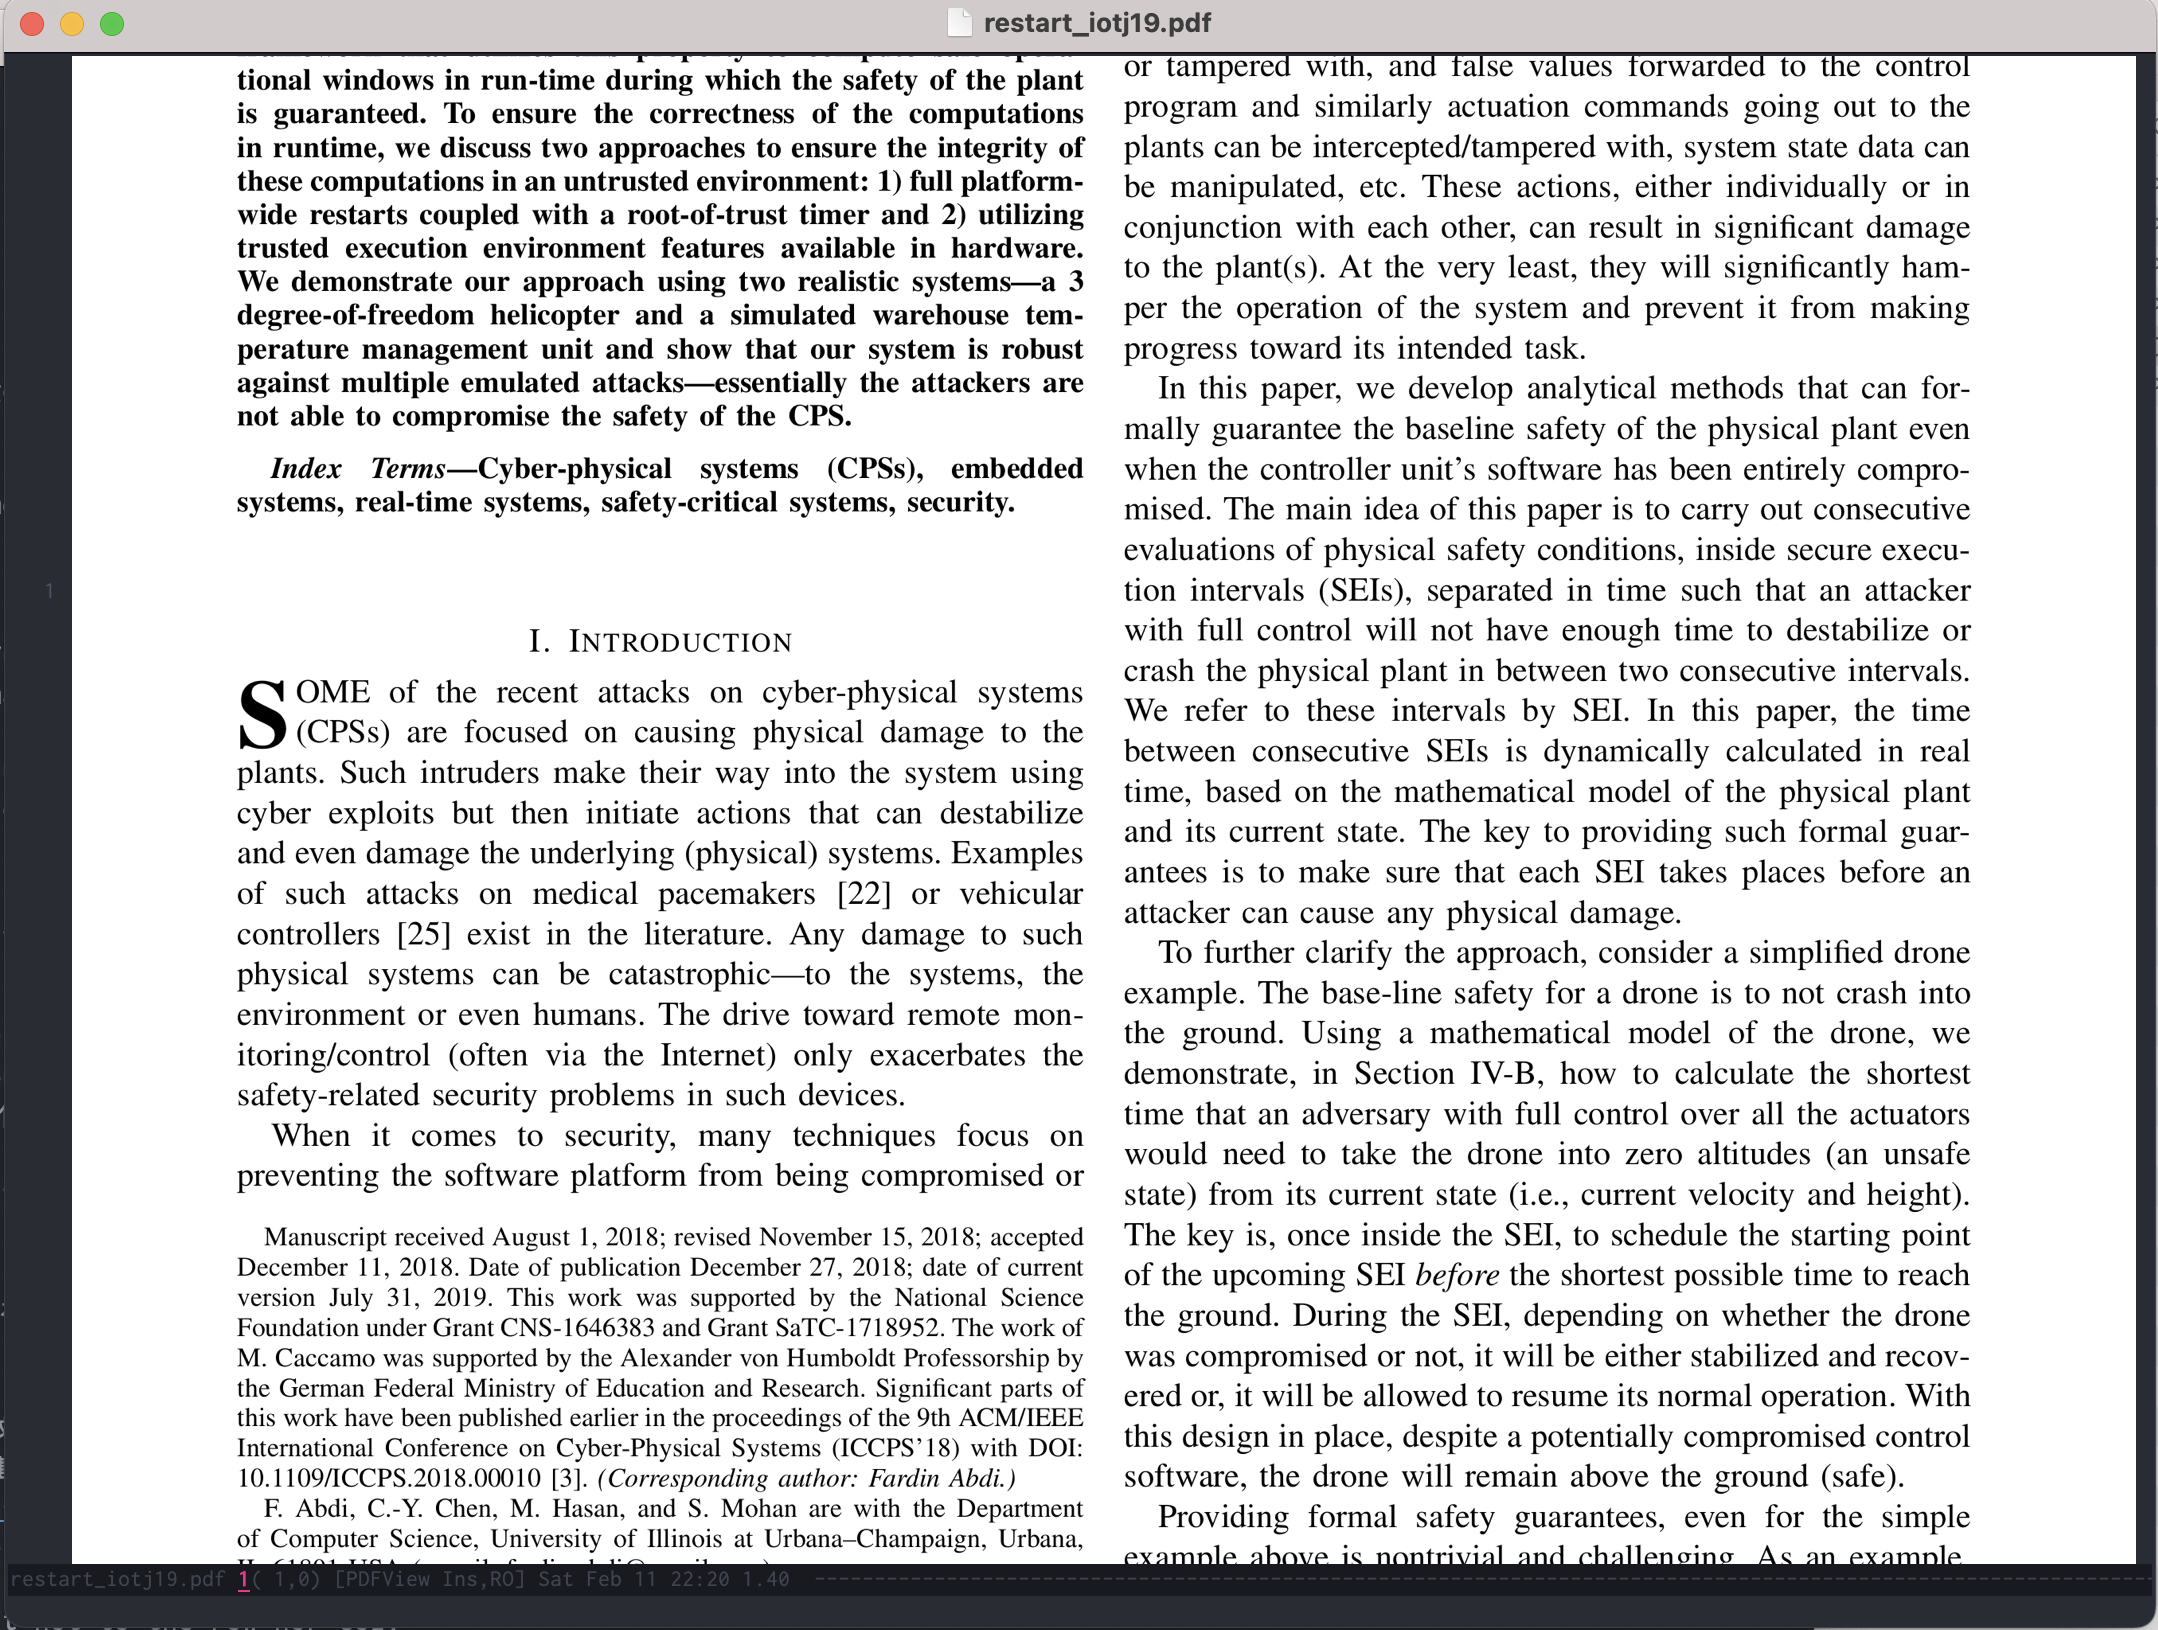
\includegraphics[width=.9\linewidth]{./pic/Snipaste_2023-02-11_22-20-25.png}
\item could customer F5 toggle sr-speedbar, and make sis-mode work. But I do NOT really need sis-mode, only needed macism command line. to help [LOVE MY DEAR COUSIN!!!]
\end{itemize}

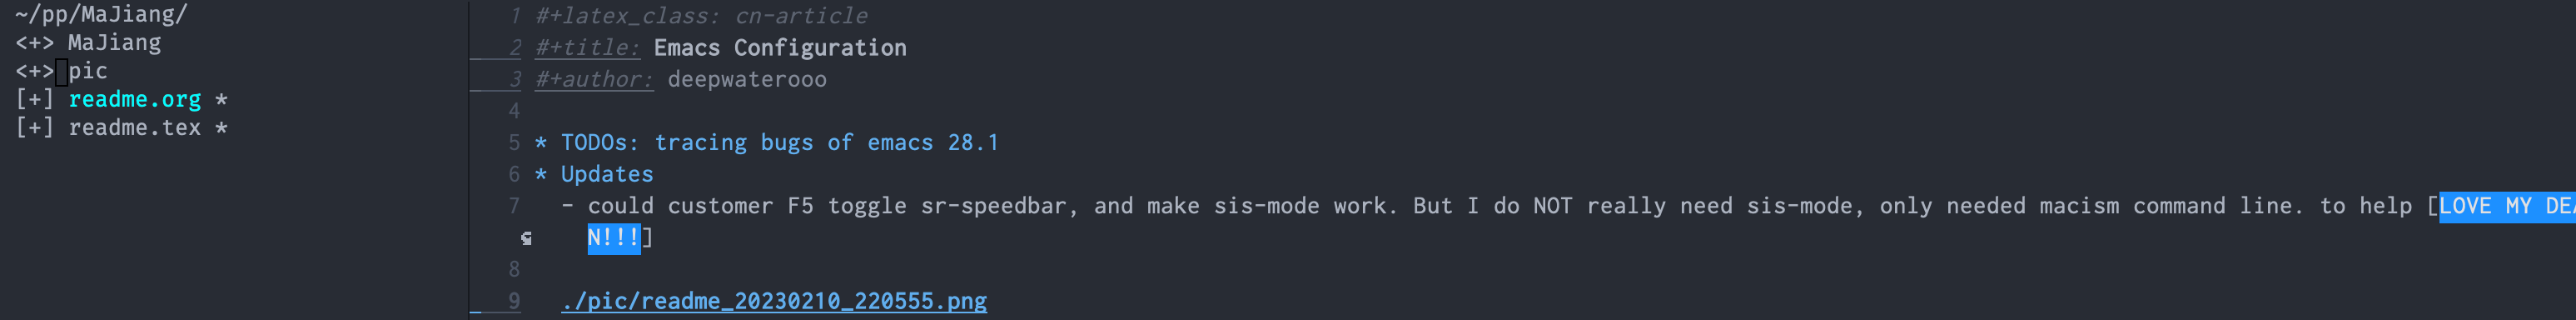
\includegraphics[width=.9\linewidth]{./pic/readme_20230210_221127.png}
\begin{itemize}
\item finally sync up with csharp-mode with tree-sitter, and fixed added the other's that gio-mode etc.
\item Permanently diabled speedbar-edit-file's set-timer function call from Resource files. Do NOT want to see such a bug, don't know how to fix, but disable it and walk around.
\item Now have a relatively barable and stable colorful emacs code editor now, at least for csharp-mode. Relatively satisfied now. Could sit it aside for a while now to focus on projects.
\end{itemize}
\subsection{invalid time specification: sr-speedbar on MacOS}
\label{sec-2-2}
\begin{itemize}
\item I don't like this bug, and I belive I do NOT really using any timer for auto-refresh in my speedbar. So I ended up by disabling the (speedbar-edit-file() func, which is frequently bug trigered) setting timer part from /Applications/Emacs.app/Contents/Resources/lisp/speedbar.el.gz, and recompile the file. The bug was gone. And I could deal with csharp-mode's fontify bug.
\item newer debugging infos, concernibg about sr-speedbar.el file. Have NOT been able to trace down for today.
\end{itemize}

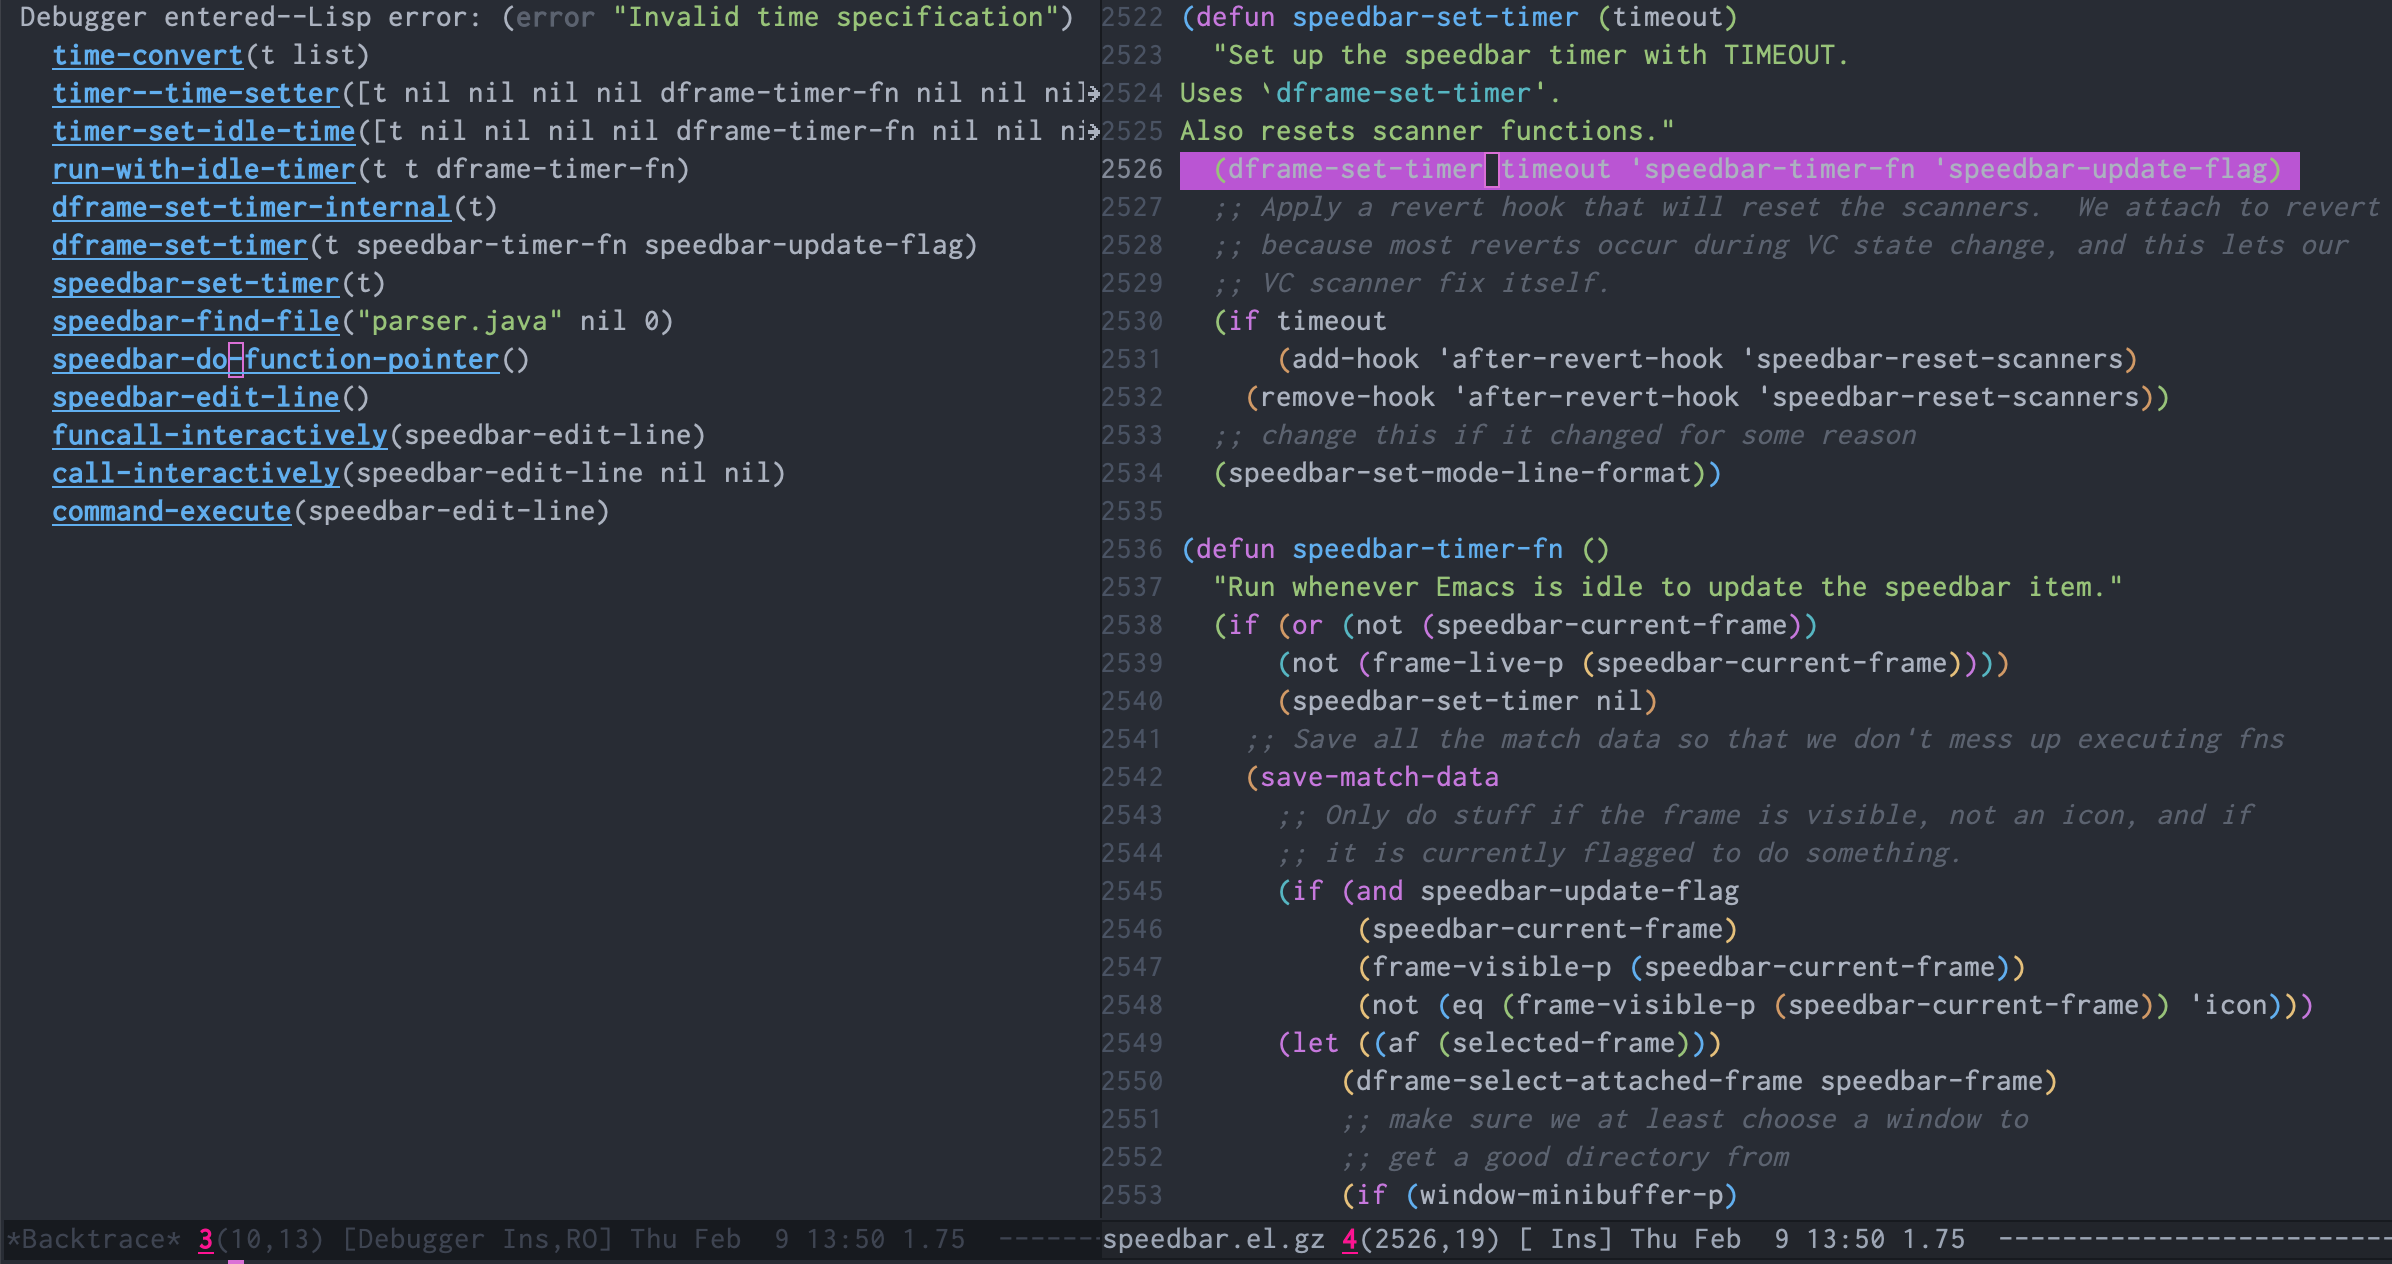
\includegraphics[width=.9\linewidth]{./pic/readme_20230209_135039.png}
\begin{itemize}
\item 好像是macOS系统常常存在的 bug,两年了关了又开,开了再关\ldots{}\ldots{}
\item \url{https://github.com/remacs/remacs/issues/845}
\item get cmake work later, not urgent though.Complete
\item babel org-mode so I don't have to copy from specific babeled source org-mode files in order for chinese characters to work.
\item Installed my emacs of version 28.1. But there is a bug of any verison emacs > 27.1, and I am NOT able to find a installable emacs 27.1 version any more.
\item 不同电脑架构上可能因为架构的不同,可以可能可以有某些优化.又照一个单做了一遍,似乎没有出错. \url{https://goykhman.ca/gene/blog/2022/2022-04-10-emacs-28.1-on-m1.html}
\item 但是我没有没能加入那个补丁包.暂时没能想好怎么加入那个补丁包. ( \textbf{todo: 改天可以尝试再把这个补丁包加进去} )
\item 因为构建是在原有现有的 mac 28.1.1版本上构建的.所以改动什么,或是不曾改变,又或者改不了不影响明显功能都是无从知晓的,但是它最后的两个步骤的验证都是成功的,应该还是构建成功了吧?
\end{itemize}

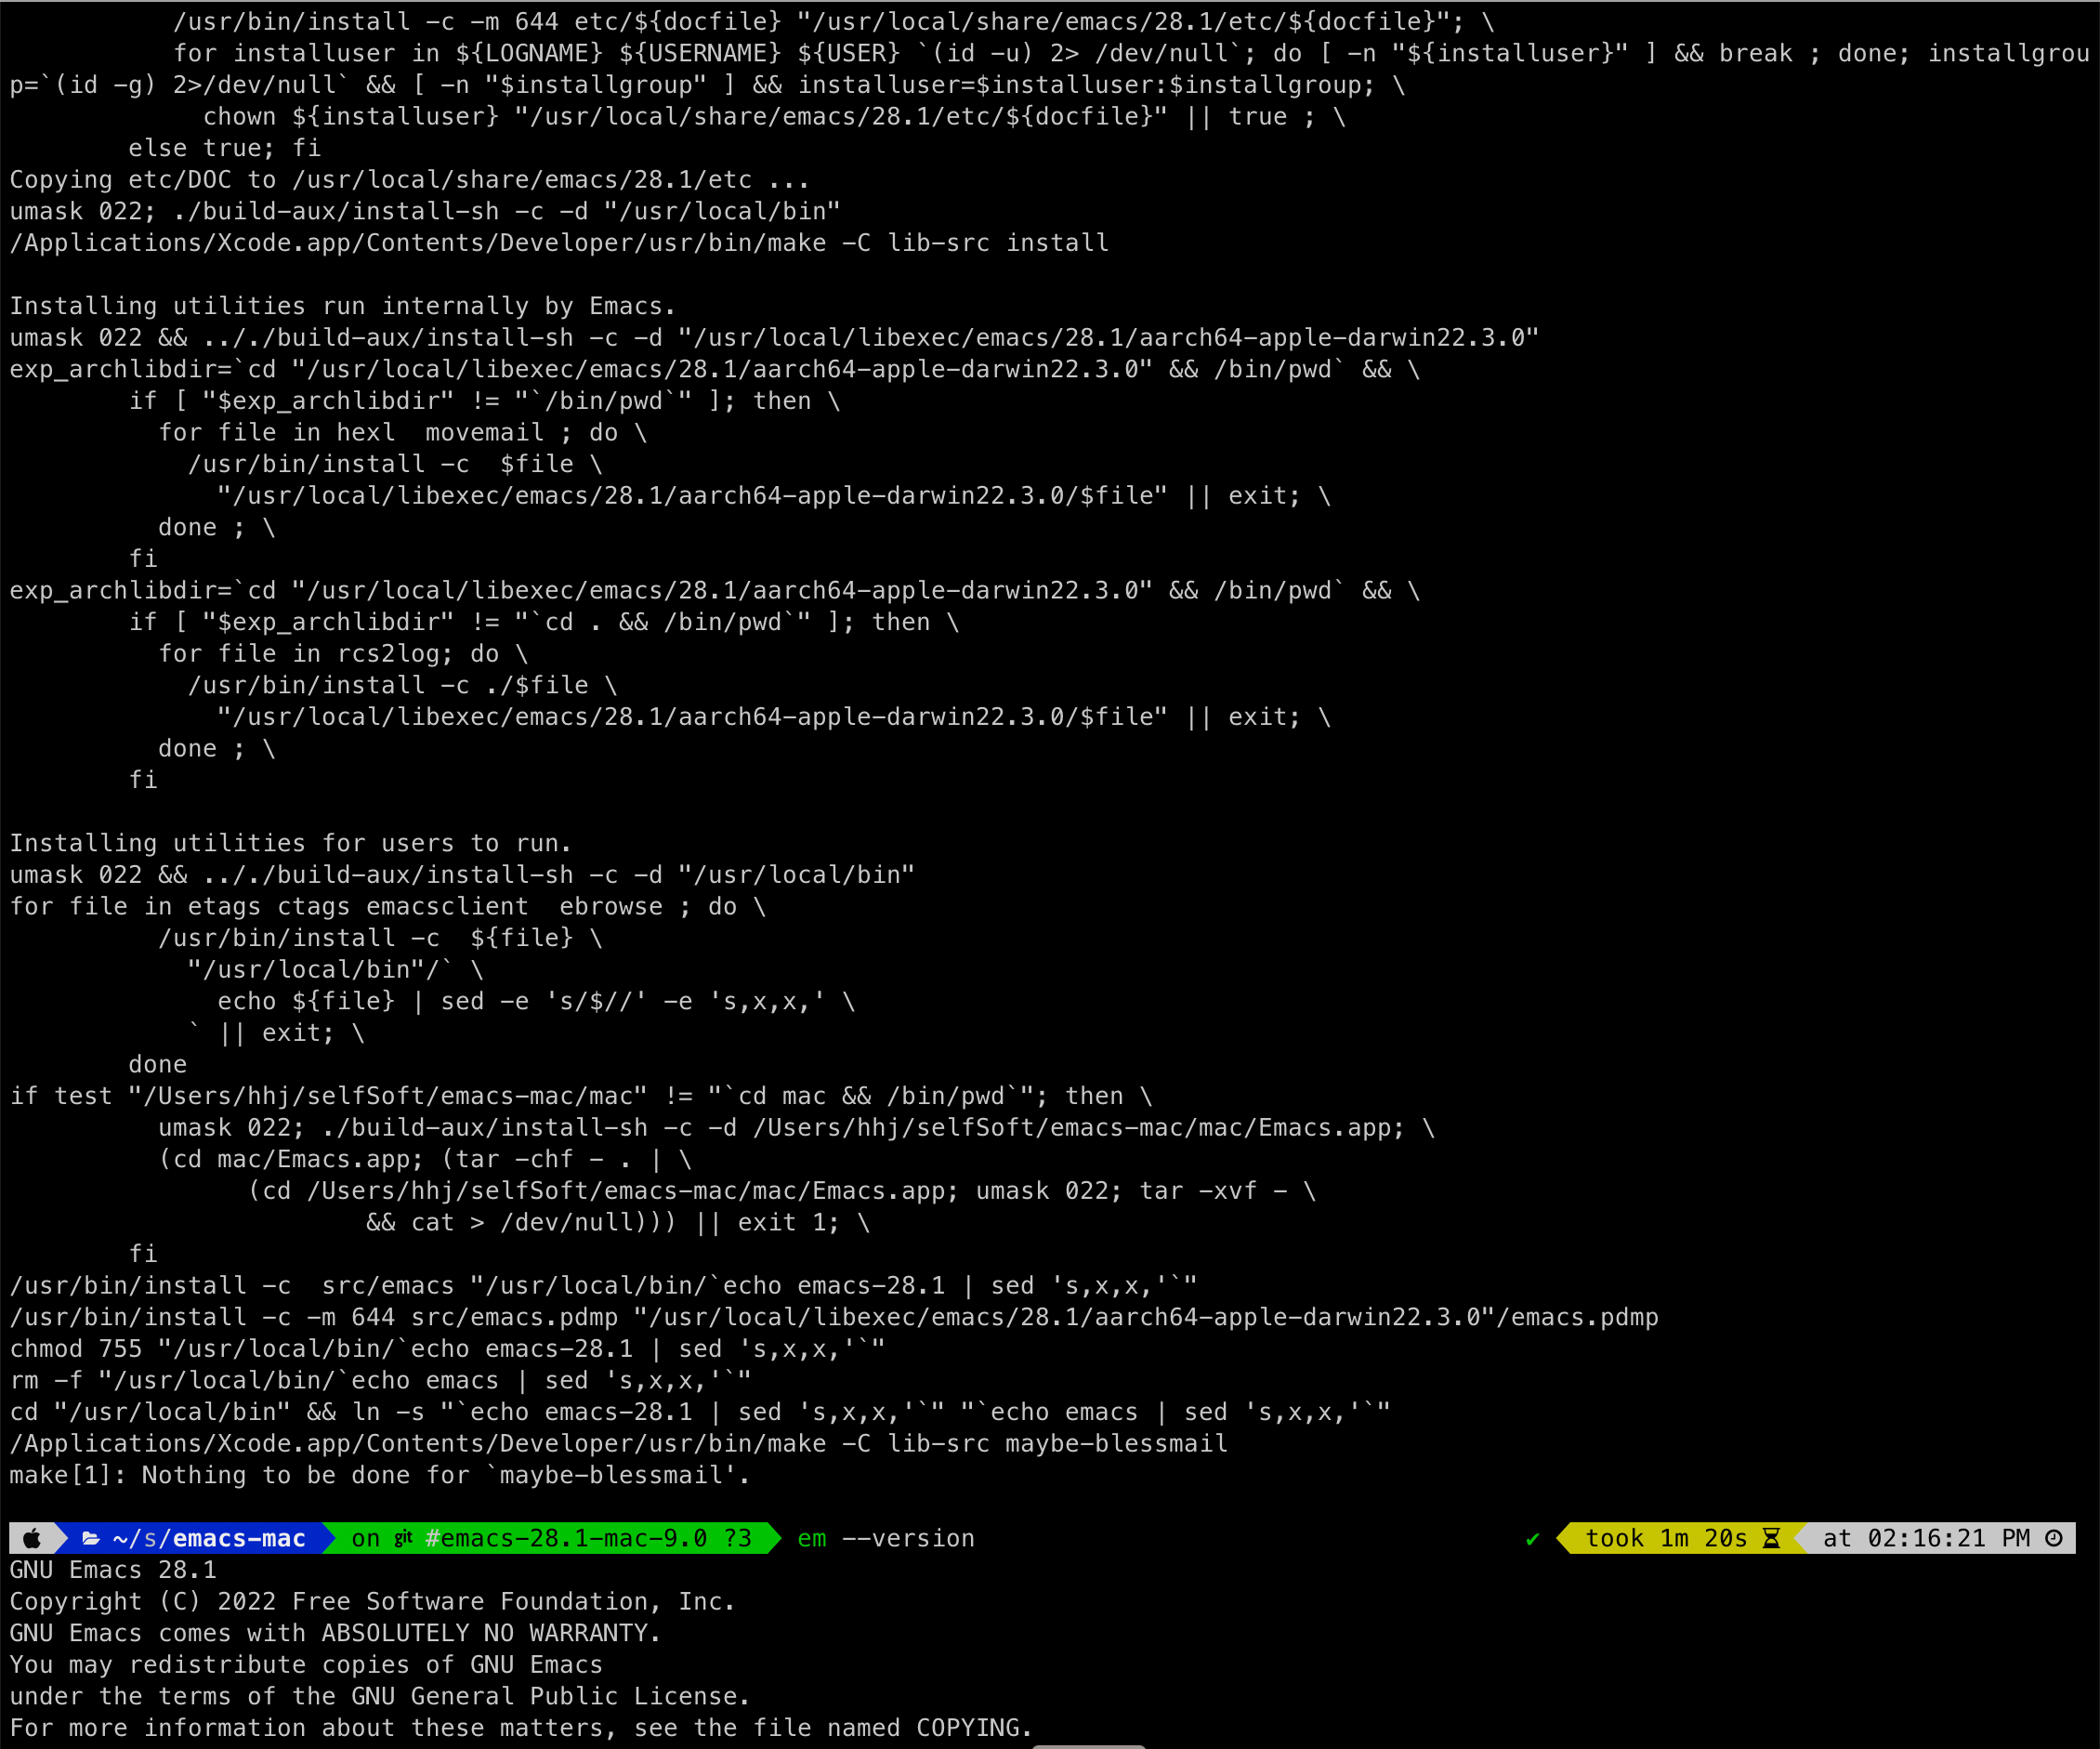
\includegraphics[width=.9\linewidth]{./pic/readme_20230208_142554.png}
\begin{itemize}
\item 今天又尝试安装Xcode之后再构建一遍,但是没有成功.可能本身参考有些年代,另外自己还完全不通这个部分,所以暂时放一放.改天有机会可以再回来研究一下,错在哪里,我如何才可能构建出自己的版本.
\end{itemize}

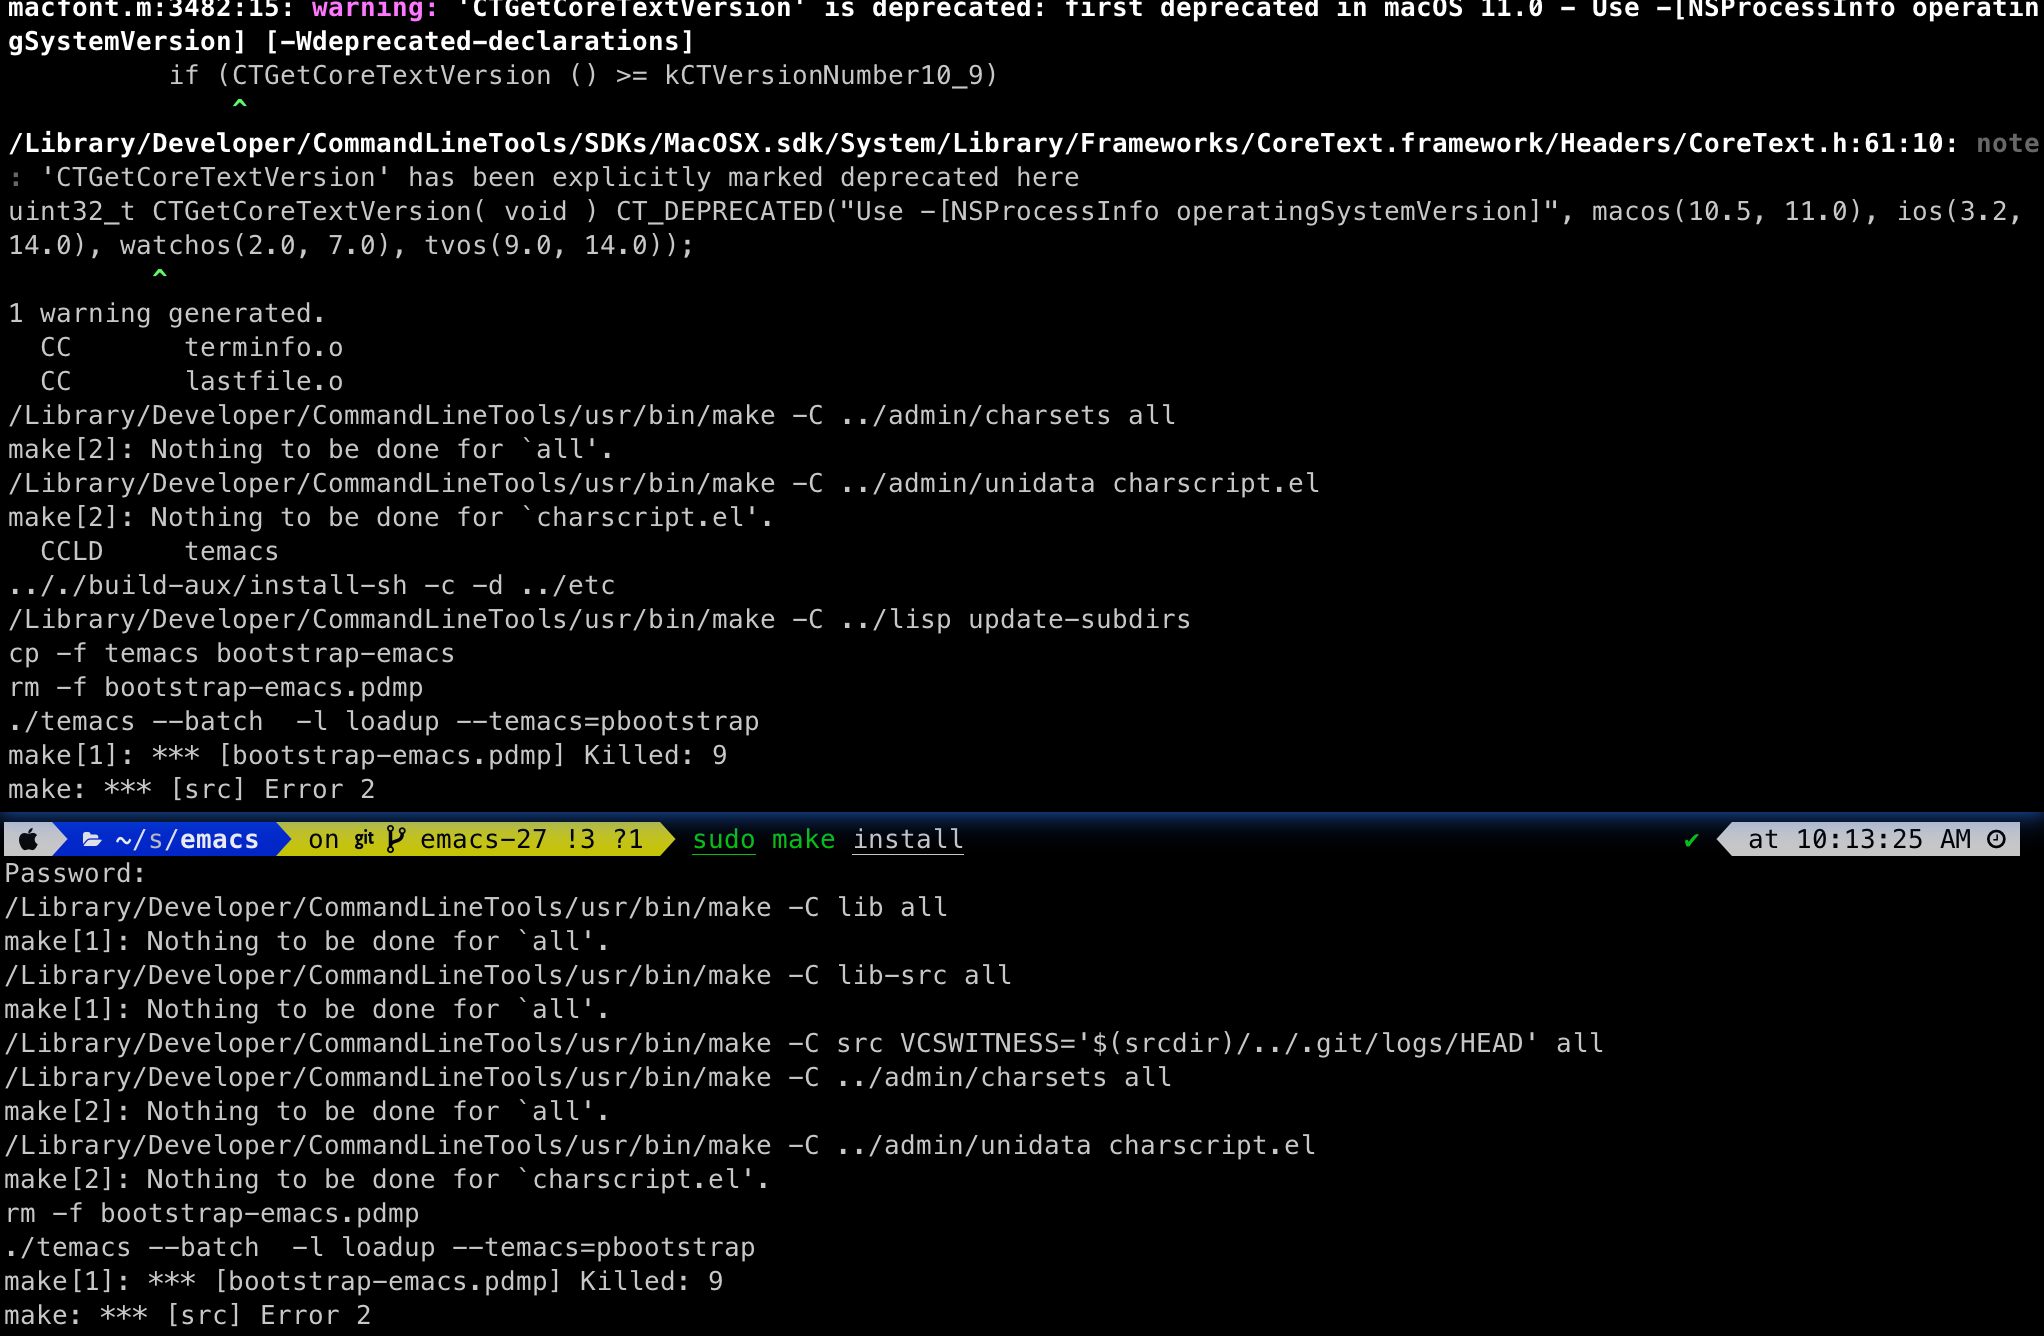
\includegraphics[width=.9\linewidth]{./pic/readme_20230208_102317.png}
\begin{itemize}
\item 上面又成为一个需要改的东西: 就是系统下如何从剪贴板自动生成写入文件 org-mode M-s
\item 然后看见这里说可以自己构建一个,连Xcode也没有安装,就跑去构建了,当然不成功。这段时间太忙,XCode要的空间太大了,暂时还不想。等改天有机会的时候倒是可以一试的
\begin{itemize}
\item \url{https://stuff-things.net/2020/12/28/building-emacs-27-dot-1-on-macos-big-sur/}
\end{itemize}
\item added key-bindings for opening from VSCode/Android Studio of current emacs buffer. 
\begin{itemize}
\item VSC Emacs can locate to each othr to correct row and col.
\item Android Studio could open current emacs buffer. but not to the row nor col.
\end{itemize}
\item I liked recently configued Visual studio 2019 one-dark-pro theme, want to configue it for emacs, but ended up with any permission denied, renaming emacs initiating bug. reverted back for daily use, and may look into that bug for later reference.
\item will reconfigure one-dark-pro theme later.
\item fixed legency java-mode highlighing issue which I did not fix for years. Has been able to treat java-mode as java-mode Instead of using it as csharp-mode. Can not separate java-mode snippets from csharp-mode's.
\end{itemize}
\subsection{BUG statement and partial fix}
\label{sec-2-3}
\begin{itemize}
\item in java-mode, the code style I expected is as followed:
\end{itemize}
\begin{minted}[fontsize=\scriptsize,linenos=false]{java}
class node {
    int v ;
    public node() {
        if (a > 0) // I don't want { } blocks when I have only one line statement inside blocks
     // a = 17;    // before fix:
            a = 17;   // now it can auto-indent
        b = 20;
        while (true)  // same auto indents here
            j++;
    }
}
class dklfjdj {|} // <<==== current un-auto-expanded version, bug right now for java-mode
class dklfjdj { 
    | // <<==== expected feature: once I typed '{', '}' will be autopaired(it does), but also auto-expand and cursor moves and indents directly to where I expect
}
\end{minted}
\begin{itemize}
\item if while if while one line statement autoindent without \{\} fixed today for java-mode, but for kotlin-mode, this bug consists, make coders/programmers nuts.
\end{itemize}
\begin{minted}[fontsize=\scriptsize,linenos=false]{java}
fun getStringLength(obj: Any): Int? {
    if (obj is String)
    return obj.length  // <<<<===== BUG: need to fix auto-indent here for if else while etc without {} 

    if (obj is String) {
        return obj.length
    }
    // 在离开类型检测分支后,`obj` 仍然是 `Any` 类型
    return null
}
fun dslfkj { // kotlin-mode, unlike java-mode, this feature works charming
    val a = 1720 
}
\end{minted}
\begin{itemize}
\item The \{|\} can NOT auto-expand still bugs me a lot, I don't want to switch back to java-mode yet unless bug fixed and it auto-pands.
\item java minor bug: Debugger entered--Lisp error: (void-function company-clear-completion-rules): this bug I will look into it recently, and expect it to be fixed so I could switch java-mode from csharp-mode as soon as possible.
\item \textbf{csharp-mode} has been the one that works perfectly for these two features, \{\} auto expand, also if while one line statement autoindent without \{\}, so I used csharp-mode as java mode.
\end{itemize}
\subsection{so far let it be this way}
\label{sec-2-4}
\begin{itemize}
\item Spent a whole day, half fixed the bug in the morning, but has broke java-mode completely and had to pull request from github once again.
\item I actually cannot stay kotlin-mode insdie csharp's, look at following indent:
\end{itemize}
\begin{minted}[fontsize=\scriptsize,linenos=false]{kotlin}
public fun thread(start: Boolean = true,
                  isDaemon: Boolean = false,
                  contextClassLoader: ClassLoader? = null,
                  name: String? = null,
                  priority: Int = -1,
                  block: () -> Unit
                  ): Thread {
    val thread = object : Thread() {
        public override fun run() {
            block()
        }
    }
    if (isDaemon) thread.isDaemon = true
                      if (priority > 0) thread.priority = priority
                                            if (name != null) thread.name = name
                                                                  if (contextClassLoader != null) thread.contextClassLoader = contextClassLoader
                                                                                                      if (start) thread.start()   
                                                                                                                     return thread
\end{minted}
\begin{itemize}
\item cause csharp-mode does not have ';' !!! so kotlin-mode stay as designed, I will have to bear the bug till I search and find good solutions.
\item Recently I have used csharp-mode less, so temportorily let java-mode and kotlin-mode stay inside csharp's for a while. And I only want to practise kotlin to get a comfortable level referring github android projects. So once I get familiar, i still mainly using java-mode insides csharp's, which could be Ok, untill I get a job, and finally settle down to work on java-mode and \{|\} auto-expandsion bug.
\item today's
\item will only update this repository when there is a need. emacs version 27.01 27.02
\item working on leetcode interview questions, so have not configued any JDK IDE within emacs nor from csharp-mode, only take full advantage of emacs snippets for java algorithm problems coding. Uploaded so far some frequently used snippets for my own references.
\item having not update this one for a while. pseudo-name .java jave-mode inside csharp-mode so that I can skip some pairs of \{ \}-s
\item java-mode csharp-mode file organiation scripts update
\item Unhighlight leading or trailing whitespace
\item org-move-tree make it slightly easier than before for manipulating small org files, and followed by integrating into one book file, and export into one pdf book. Seek for auto-updating integrated book file according to small chapter file updates later on when get spare time.
\item fixed emacs org-mode export to pdf broken environment for personal laptop.
\item configured company jedi environment for python3.
\item Adding snippets for csharp-mode when debugging unity games.
\item Remove not frequently used bothering commands from syslog-mode, and define simplified customized macro command for android SDK log analysis.
\item \textbf{Enhanced syslog-mode}, with simplified textile-mode feature integrated for personal debugging log viewing propose. Will continuously improve relative features.
\item logview-mode, log4j-mode, syslog-mode, in progress, so far only syslog-mode works, needs to combine textile-mode functions/hooks.
\item textile-mode for android logs;
\item sr-speedbar set fixed hight and width cater to current project file names length;
\item fixed previously existing tab cannot indent line and region problem;
\item company mode works convenient and as I expected;
\item C-c f formating files according to needs. Fix minor bugs for java python csharp-mode swift-mode auto complete.
\item clean auto-complete-mode, made repository more consistant.
\item csharp-mode: fixed minor bugs for autopairing, as well as expand \{\} for function scope.
\item swift-mode using swift3
\item org-mode src code highlight is on, just I forgot to specify language before.
\item emacs key-bound for mac keyboard, so that it would be convenient for me to type some specific keys. 
\begin{itemize}
\item exchanged the position of \^{}Control and Capslock;
\item exchanged the position of Option and Command keys;
\item through mac system preference.
\item I tried this yesterday, but after having used window's keyboard for all these years for emacs, it is still very difficult to get used to the mac keyboard even after key exchanges.
\item changed keyboard today actually so that I could type more conveniently.
\end{itemize}
\item other major-modes, for example: \textbf{java-mode}, \textbf{csharp-mode}, which I would need to use pretty soon, is ready for use now (auto-complete + yasnippet etc).
\item All the minor warnings, warning messages when starting emacs, modes fixes are all fixed, a clean Emacs open ready for work.
\end{itemize}
\section{starting point}
\label{sec-3}
\begin{itemize}
\item It is a new computer, and I did try to git clone from my own repository to new laptop, but after fixed errors and tried, \textbf{I promise I do NOT and can NOT bare the out-dated emacs 22.X any more, I have to move on.} I have to install newer versions for my own later on convenience.
\item Instead of configuring my own again, this time, I tried from some "big" person's repository and try to make it work on my laptop (fixing errors, installing necessary packages etc), as well as comment out some complicated modes and customization so that I would still be able to use and like my current emacs interface.
\item It is the first time I tried from some big person's (or any person's configurature completely), it was tidious to fix all the errors at beginning (I spent more than 2 days on it last week. For me it just took too much time), but so far I like some of the features that had been annoying me before, but I have not and was not able to find good solutions to solve it, like how to auto-complete words when in scripte comment line or in quotes. I like these detailed features which I did try by writing my own snippets from yasnippet mode before.
\item So far, org-mode is not perfect, but it is a fully functional one that I could use and help convenient a game developer's daily work.
\item Will devote more time to understand emacs better, and to solve my own problems and make it more convenient for me to use when I need some specific features.
\end{itemize}
\section{References}
\label{sec-4}
\begin{itemize}
\item \url{https://github.com/redguardtoo/emacs.d}
\end{itemize}
% Emacs 28.1 (Org mode 8.2.7c)
\end{document}